%!TEX root = practicum3.tex
\subsection*{Point in Triangle}

% Theory
We try to determine if the point \vec{Q} lies in the triangle defined by the points $\vec{P_1}$, $\vec{P_2}$ and $\vec{P_3}$. To this end we define the vectors $\vec{v}_1 = \vec{P_2} - \vec{P_1}$ and $\vec{v_2} = \vec{P_3} - \vec{P_1}$, see \autoref{fig:a:triangle_point}. Each point $\vec{P}$ inside the grey area in this figure can be described as:
\begin{equation} \label{eq:a:trianglePointEquation}
	\vec{P} = \vec{P_1} + a \cdot \vec{v_1} + b \cdot \vec{v_2}.
\end{equation}
For all points to the right of \vec{P_1} $a > 0$ and $b > 0$. The points that define the triangle can all be expressed according to \eqref{eq:a:trianglePointEquation}:
\begin{align}
	\vec{P_1} &= \vec{P_1} + 0 \cdot \vec{v_1} + 0 \cdot \vec{v_2} \label{eq:a:p1}\\ 
	\vec{P_2} &= \vec{P_1} + 1 \cdot \vec{v_1} + 0 \cdot \vec{v_2} \label{eq:a:p2}\\ 
	\vec{P_3} &= \vec{P_1} + 0 \cdot \vec{v_1} + 1 \cdot \vec{v_2} \label{eq:a:p3}.
\end{align}
Based on these \eqref{eq:a:p1} through \eqref{eq:a:p3} we find that a point \vec{Q} lies on the triangle if it can be expressed according to \eqref{eq:a:trianglePointEquation} with $a,b \in (0,1)$ and with $a + b < 1$. 

Solving the resulting equation with Mathematica, see \autoref{lst:a:pointInTriangleMathematica}, gives us expressions for $a$ and $b$, namely:
	\begin{align}
	a &= -\frac{-\vec{p_{10}} \vec{p_{31}}+\vec{p_{10}} \vec{Q1}+\vec{p_{11}} \vec{p_{30}}-\vec{p_{11}}
   \vec{Q0}-\vec{p_{30}} \vec{Q1}+\vec{p_{31}} \vec{Q0}}{-\vec{p_{10}}
   \vec{p_{21}}+\vec{p_{10}} \vec{p_{31}}+\vec{p_{11}} \vec{p_{20}}-\vec{p_{11}}
   \vec{p_{30}}-\vec{p_{20}} \vec{p_{31}}+\vec{p_{21}} \vec{p_{30}}}\\
	b &= -\frac{-\vec{p_{10}} \vec{p_{21}}+\vec{p_{10}} \vec{Q1}+\vec{p_{11}} \vec{p_{20}}-\vec{p_{11}}
   \vec{Q0}-\vec{p_{20}} \vec{Q1}+\vec{p_{21}} \vec{Q0}}{\vec{p_{10}}
   \vec{p_{21}}-\vec{p_{10}} \vec{p_{31}}-\vec{p_{11}} \vec{p_{20}}+\vec{p_{11}}
   \vec{p_{30}}+\vec{p_{20}} \vec{p_{31}}-\vec{p_{21}} \vec{p_{30}}}
	\end{align}

	\begin{lstlisting}[float, language=Mathematica, label={lst:a:pointInTriangleMathematica}, caption={Mathematica code used to compute the to compute $a$ and $b$.}]
p1 = {p10, p11};
p2 = {p20, p21};
p3 = {p30, p31};
v1 = p2 - p1;
v2 = p3 - p1;

p4 = p1 + a * v1 + b * v2;
p41 = Part[p4, 1] == Q0;
p42 = Part[p4, 2] == pp1;
solution = Solve[{p41, p42}, {a, b}]
	\end{lstlisting}

\begin{figure}
	\centering
	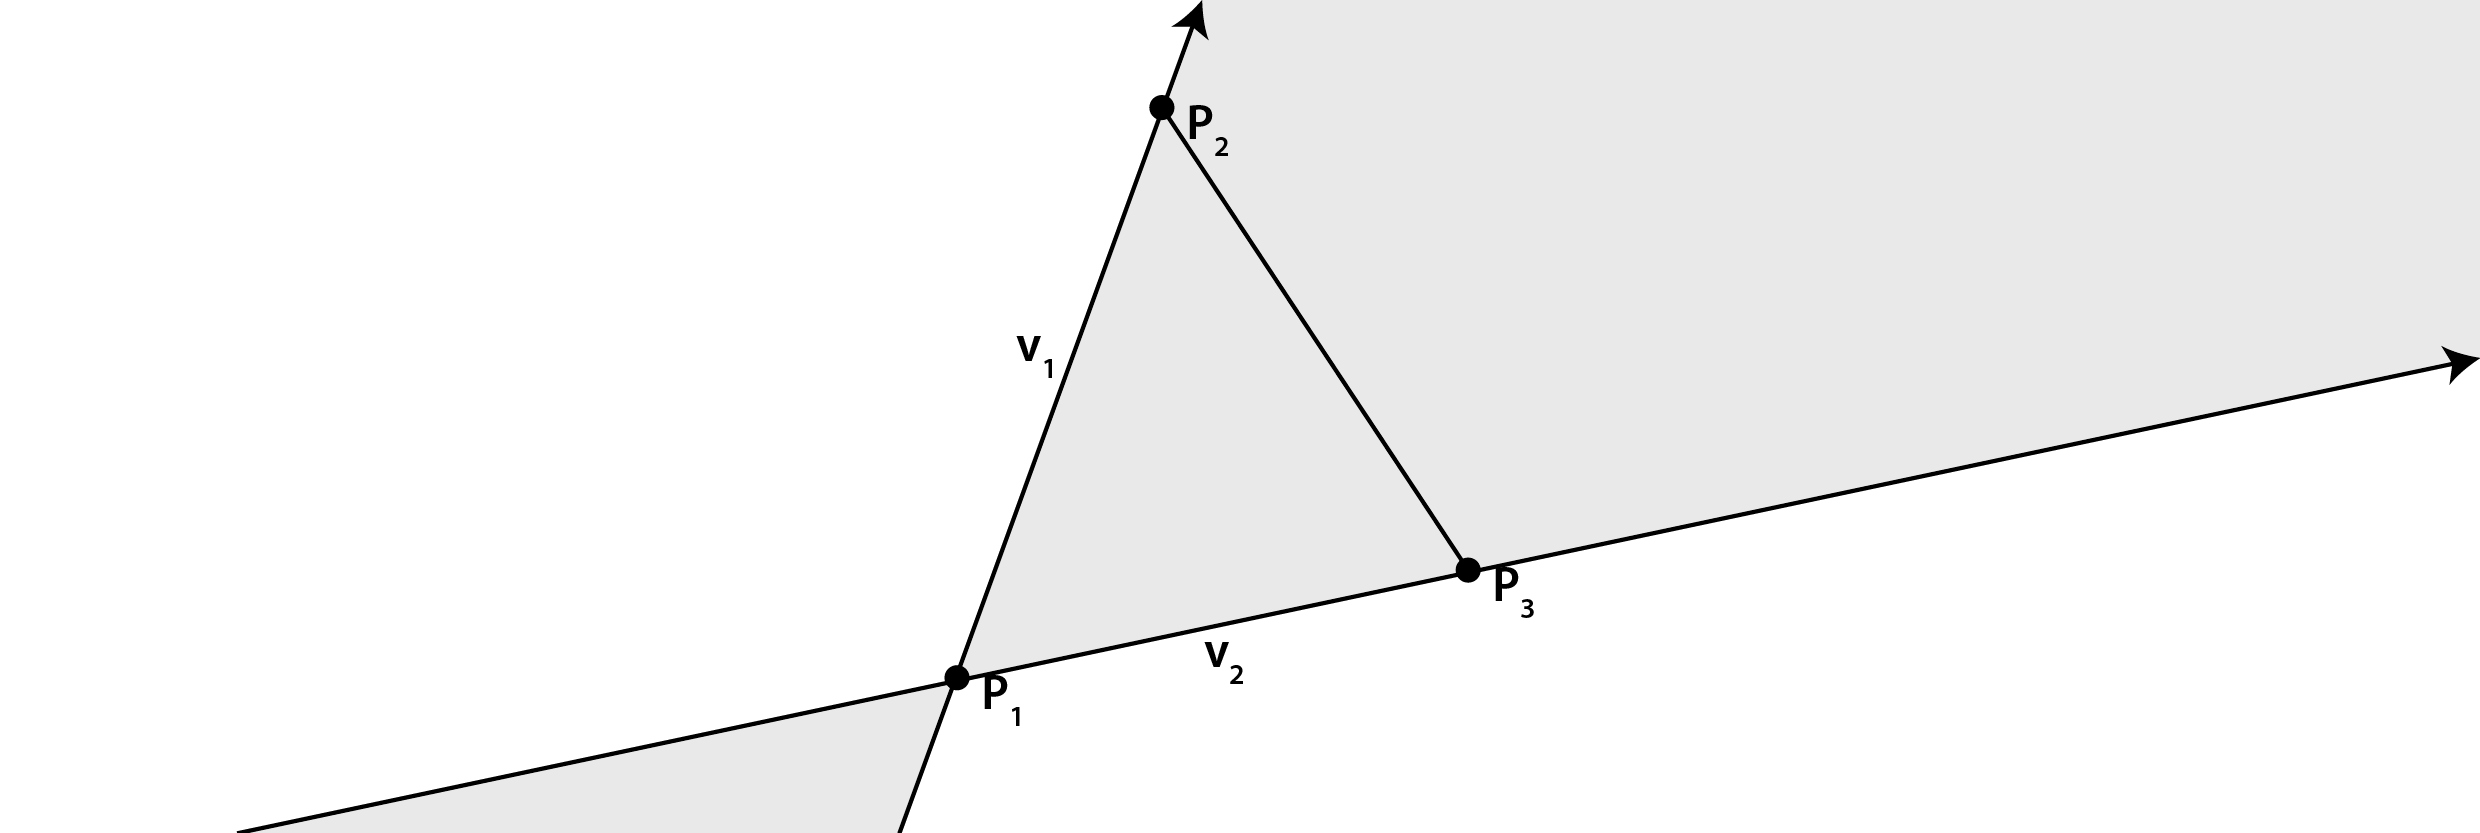
\includegraphics[width=0.9\textwidth, frame]{./img/1_triangle_point-01}
	\caption{A triangle defined by the points $\vec{P_1}$, $\vec{P_2}$ and $\vec{P_3}$, with the vectors $\vec{v_1}$ and $\vec{v_2}$. The grey area covers all points that can be described according to \eqref{eq:a:trianglePointEquation}.}
	\label{fig:a:triangle_point}
\end{figure}




\subsection{Finding the Triangle}
